\newpage
\chapter{TINJAUAN PUSTAKA} \label{Bab II}

\section{Tinjauan Pustaka} \label{II.Tinjauan}
Tinjauan pustaka berikut memaparkan berbagai penelitian terdahulu yang memiliki relevansi dengan topik yang diteliti serta menjadi landasan utama dalam penyusunan tugas akhir. Kajian ini bertujuan untuk memberikan gambaran mengenai perkembangan penelitian yang berkaitan dengan permasalahan yang diteliti. Selain itu, tinjauan pustaka juga membantu dalam mengidentifikasi kelebihan dan keterbatasan dari penelitian sebelumnya. Adapun penelitian-penelitian yang dijadikan sebagai acuan utama diuraikan sebagai berikut.

Penelitian yang dilakukan oleh Sharma et al. pada tahun 2022 menyajikan sebuah studi tinjauan yang mengkaji perkembangan penelitian terkait meme berbahaya beserta tantangan yang dihadapi dalam bidang tersebut. Melalui analisis terhadap berbagai penelitian sebelumnya, penulis mengidentifikasi bahwa sebagian besar studi masih berfokus pada kategori meme tertentu, sementara jenis meme lain seperti yang berkaitan dengan \textit{self-harm} belum banyak diteliti. Temuan utama dari penelitian ini menunjukkan bahwa keterbatasan ketersediaan dataset menjadi faktor utama yang menghambat eksplorasi pada kategori tersebut \cite{Sharma2022HarmfulMemes}. Oleh karena itu, penelitian ini menegaskan adanya kesenjangan riset yang signifikan, khususnya dalam penyediaan dataset dan pengembangan metode untuk analisis meme \textit{self-harm}.

Penelitian yang dilakukan oleh Pramanick \textit{et al.} pada tahun 2021 memperkenalkan MOMENTA, yaitu sebuah kerangka kerja multimodal yang dirancang untuk mendeteksi meme berbahaya sekaligus mengidentifikasi target yang disasar. Metode yang diusulkan menggabungkan informasi global melalui representasi gabungan gambar dan teks, serta informasi lokal yang diperoleh dari deteksi objek, atribut visual, dan ekstraksi teks menggunakan \textit{Optical Character Recognition} (OCR), sehingga mampu menangkap konteks meme secara lebih komprehensif. Hasil eksperimen menunjukkan bahwa MOMENTA mampu mengungguli berbagai model pembanding pada tugas deteksi meme berbahaya dan identifikasi target, dengan peningkatan performa yang konsisten \cite{pramanick2021momenta}. Meskipun penelitian ini berfokus pada kategori \textit{hate speech} dan propaganda, pendekatan multimodal yang digunakan menunjukkan relevansi untuk analisis meme \textit{self-harm}, sekaligus mengindikasikan adanya peluang pengembangan lebih lanjut pada kategori tersebut yang masih belum banyak diteliti.

Penelitian yang dilakukan oleh Kumar dan Nandakumar pada tahun 2022 mengusulkan Hate-CLIPper, yaitu model klasifikasi meme berbasis multimodal yang memanfaatkan representasi dari CLIP serta interaksi eksplisit antara fitur visual dan teks. Penelitian ini dilatarbelakangi oleh permasalahan bahwa informasi pada meme tidak dapat dipahami secara terpisah antara gambar dan teks, sehingga diperlukan pemodelan hubungan lintas-modal yang lebih efektif . Untuk mengatasi hal tersebut, penulis memperkenalkan \textit{feature interaction matrix} yang dibangun dari interaksi antara \textit{embedding}  visual dan teks, sehingga mampu menangkap hubungan semantik secara lebih mendalam dibandingkan pendekatan konvensional . Hasil eksperimen menunjukkan bahwa model yang diusulkan mencapai performa \textit{state-of-the-art} dengan nilai AUROC sebesar 85{,}8\% pada dataset Hateful Memes Challenge, bahkan melampaui performa manusia, serta menunjukkan kemampuan generalisasi pada dataset lain \cite{kumar2022hateclipper}. Meskipun penelitian ini berfokus pada deteksi hate speech, pendekatan berbasis interaksi fitur lintas-modal yang diusulkan memberikan dasar yang kuat untuk menangkap makna implisit pada meme, sehingga membuka peluang penerapan pada analisis meme \textit{self-harm} yang masih terbatas dalam penelitian sebelumnya.

Penelitian yang dilakukan oleh Shah \textit{et al.} pada tahun 2024 mengusulkan \textit{MemeCLIP}, yaitu sebuah \textit{framework} multimodal yang memanfaatkan representasi CLIP untuk melakukan klasifikasi meme secara multiaspek. Penelitian ini dilatarbelakangi oleh keterbatasan studi sebelumnya yang umumnya hanya berfokus pada satu aspek, seperti \textit{hate speech}, sehingga belum mampu menangkap kompleksitas makna dalam meme yang bersifat multi-dimensi. Untuk mengatasi hal tersebut, penulis memperkenalkan dataset baru bernama \textit{PrideMM} yang terdiri dari 5.063 meme terkait gerakan \textit{LGBTQ+} dengan beberapa label sekaligus, yaitu \textit{hate}, \textit{target}, \textit{stance}, dan \textit{humor}, serta mengembangkan pendekatan berbasis CLIP yang diadaptasi untuk pembelajaran \textit{downstream}. Hasil eksperimen menunjukkan bahwa \textit{MemeCLIP} mampu mengungguli berbagai metode sebelumnya pada beberapa dataset nyata, serta menunjukkan performa yang kompetitif ketika dibandingkan dengan pendekatan \textit{zero-shot} berbasis \textit{GPT-4} \cite{shah2024memeclip}. Temuan ini menegaskan pentingnya pendekatan multiaspek dalam analisis meme, sekaligus menunjukkan adanya peluang penelitian lebih lanjut untuk memasukkan kategori lain seperti \textit{self-harm} yang belum tercakup dalam skema klasifikasi tersebut.

Penelitian yang dilakukan oleh Lian \textit{et al.} pada tahun 2023 mengevaluasi kemampuan model multimodal \textit{GPT-4V} dalam tugas pengenalan emosi secara luas melalui pendekatan \textit{zero-shot}. Dalam penelitian tersebut, penulis menyusun 21 dataset \textit{benchmark} yang mencakup berbagai tugas emosi, seperti analisis sentimen pada gambar dan teks, serta pengenalan ekspresi wajah dalam kondisi statis maupun dinamis. Hasil eksperimen menunjukkan bahwa \textit{GPT-4V} memiliki kemampuan yang kuat dalam memahami informasi visual dan emosional, serta mampu memanfaatkan petunjuk multimodal dan konteks temporal, meskipun masih memiliki keterbatasan dalam mengenali ekspresi mikro yang sangat spesifik \cite{lian2023gpt4v}. Temuan ini menunjukkan potensi \textit{large multimodal models} sebagai alat anotasi otomatis tanpa memerlukan pelatihan tambahan, sehingga relevan untuk mengatasi keterbatasan dataset pada penelitian meme \textit{self-harm} melalui pendekatan anotasi berbasis model multimodal.


Penelitian-penelitian yang menjadi referensi penulis dijabarkan pada Tabel \ref{table:2.literasi} di bawah ini. \par

\begin{landscape}
\begin{table}[H]
    \centering
    \caption{Literasi Penelitian Terdahulu}
    \label{table:2.literasi}
    \small
    \setlength{\tabcolsep}{4pt}
    \renewcommand{\arraystretch}{1.2}
    \begin{tabular}{>{\raggedright\arraybackslash}m{0.4cm} >{\raggedright\arraybackslash}m{1.6cm} >{\raggedright\arraybackslash}m{3cm} >{\raggedright\arraybackslash}m{2.8cm} >{\raggedright\arraybackslash}m{3cm} >{\raggedright\arraybackslash}m{3.8cm}}
        \hline
        \textbf{No.} & \textbf{Peneliti} & \textbf{Judul} & \textbf{Permasalahan} & \textbf{Metode} & \textbf{Hasil} \\
        \hline
        1. & Sharma \textit{et al.} (2022) \cite{Sharma2022HarmfulMemes} & \textit{Detecting and Understanding Harmful Memes: A Survey} & Minimnya studi untuk meme berbahaya termasuk \textit{self-harm} & Survei literatur dan klasifikasi tipologi meme berbahaya & Menyoroti gap penting yaitu meme \textit{self-harm} belum diteliti dan sulit karena data tidak tersedia \\
        \hline
        2. & Pramanick \textit{et al.} (2021) \cite{pramanick2021momenta} & \textit{MOMENTA: Multimodal Framework for Harmful Memes} & Deteksi meme toksik dan targetnya (menggabungkan konteks visual + teks) & \textit{Framework} multimodal MOMENTA: gabungkan fitur global (CLIP) dan lokal (wajah/objek via VGG-19 + OCR) dengan \textit{attention fusion} & Kinerja unggul, yaitu akurasi +1,3--2,6 poin dibanding \textit{baseline} dengan dua tugas, yaitu deteksi bahaya dan identifikasi target \\
        \hline
        3. & Kumar \& Nandakumar (2022) \cite{kumar2022hateclipper} & \textit{Hate-CLIPper: Multimodal Hateful Meme Classification based on Cross-modal Interaction of CLIP Features} & Klasifikasi meme kebencian dengan interaksi fitur halus & Arsitektur Hate-CLIPper: menggunakan \textit{embedding} CLIP (gambar dan teks) dan \textit{Feature Interaction Matrix} (\textit{outer-product}) & AUROC 85,8\% pada dataset Hateful Memes (melampaui manusia 82,65\%); generalis di beberapa dataset meme lainnya \\
        \hline
    \end{tabular}
\end{table}

\vspace{0.5cm}

\vspace*{1cm}
\begin{table}[H]
    \centering
    \caption{Literasi Penelitian Terdahulu}
    \label{table:2.literasi.2}
    \small
    \setlength{\tabcolsep}{4pt}
    \renewcommand{\arraystretch}{1.2}
    \begin{tabular}{>{\raggedright\arraybackslash}m{0.4cm} >{\raggedright\arraybackslash}m{1.6cm} >{\raggedright\arraybackslash}m{3cm} >{\raggedright\arraybackslash}m{2.8cm} >{\raggedright\arraybackslash}m{3cm} >{\raggedright\arraybackslash}m{3.8cm}}
        \hline
        \textbf{No.} & \textbf{Peneliti} & \textbf{Judul} & \textbf{Permasalahan} & \textbf{Metode} & \textbf{Hasil} \\
        \hline
        4. & Shah \textit{et al.} (2024) \cite{shah2024memeclip} & \textit{MemeCLIP: CLIP for Multimodal Meme Classification} & Klasifikasi meme multimodal dengan label multiperkara (\textit{hate}, \textit{target}, \textit{humor}) & Dataset baru PrideMM (5.063 meme LGBT) dengan label \textit{hate}/\textit{target}/\textit{stance}/\textit{humor}; melatih CLIP dengan adapter ringan & MemeCLIP unggul pada dua dataset nyata (PrideMM dan HarMeme) dibanding metode sebelumnya \\
        \hline
        5. & Lian \textit{et al.} (2023) \cite{lian2023gpt4v} & \textit{GPT-4V with Emotion: Zero-shot Benchmark for Emotion Recognition} & Evaluasi GPT-4V di tugas pengenalan emosi multimodal & Uji \textit{zero-shot} GPT-4V pada 21 dataset emosi (visual + teks) termasuk analisis sentimen dan ekspresi wajah & GPT-4V kuat di tugas emosi umum dan integrasi multimodal baik, namun lemah mengenali ekspresi mikro khusus \\
        \hline
    \end{tabular}
\end{table}
\end{landscape}




\section{Dasar Teori} \label{II.teori}
Berikut adalah penjelasan mengenai teori-teori yang menjadi landasan dalam penelitian ini, termasuk konsep-konsep utama seperti \textit{self-harm}, meme, multimodal \textit{deep learning}, klasifikasi \textit{fusion}, \textit{computer vision}, \textit{natural language processing}, \textit{deep learning}, \textit{transformer}, \textit{Contrastive Language-Image Pre-training} (CLIP) dan \textit{Efficiently and Encoder that Classifies Token Replacements Accurately} (ELECTRA). Penjelasan ini bertujuan untuk memberikan pemahaman yang mendalam mengenai konsep-konsep tersebut serta bagaimana mereka saling terkait dalam penelitian ini.

\subsection{\textit{Self-Harm}} \label{II.teori10}
\textit{Self-harm} atau perilaku menyakiti diri sendiri merupakan tindakan yang dilakukan seseorang untuk melukai tubuhnya secara sengaja, baik dengan maupun tanpa niat untuk mengakhiri hidup. \textit{World Health Organization} (WHO) mendefinisikan \textit{self-harm} sebagai \textit{ ``intentional self-inflicted injury, with or without suicidal intent''} \cite{WHO2014PreventingSuicide}. Dalam ranah psikiatri, DSM-5 (\textit{Diagnostic and Statistical Manual of Mental Disorders} edisi kelima) membedakan antara \textit{non-suicidal self-injury} (NSSI), yaitu perilaku menyakiti diri tanpa niat bunuh diri yang setidaknya terjadi selama lima hari dalam setahun, dengan \textit{suicidal behavior} yang berorientasi pada keinginan mengakhiri hidup \cite{APA2022_DSM5TR}. \textit{Self-harm} banyak dikaitkan dengan kondisi psikologis seperti depresi, kecemasan, dan kesulitan regulasi emosi \cite{Sabrina2023DisregulasiEmosi}.

Berdasarkan penelitian Marchant \textit{et al.} pada tahun 2017, \textit{self-harm} dalam konten digital didefinisikan sebagai fenomena yang mencakup penyebaran gambar atau video eksplisit mengenai tindakan melukai diri sendiri, serta pemanfaatan platform daring untuk mengomunikasikan distres psikologis, keputusasaan, dan ide bunuh diri, khususnya kepada rekan sebaya. Konten digital ini sering kali berperan dalam menormalisasi perilaku menyakiti diri sebagai mekanisme koping yang dianggap efektif. Selain itu, konten tersebut juga dapat menyediakan informasi teknis terkait metode pelukaan dan cara penyembunyiannya, serta berpotensi menimbulkan efek pemicu  maupun kompetisi di antara individu yang rentan \cite{Marchant2017}.

Perkembangan media sosial memperluas cara individu mengekspresikan pikiran atau perasaan terkait \textit{self-harm}. Penelitian menunjukkan bahwa konten \textit{self-harm} di platform digital seperti Instagram, TikTok, dan Reddit sering muncul dalam bentuk teks, gambar, atau kombinasi keduanya, dan dapat menjadi indikator risiko ideasi bunuh diri maupun NSSI pada remaja dan dewasa muda \cite{arendt2019effects}. Paparan konten tersebut dapat meningkatkan risiko perilaku, normalisasi \textit{self-harm}, serta perburukan kondisi mental pengguna yang rentan. Bentuk ekspresi \textit{self-harm} di media sosial sering kali bersifat implisit melalui humor gelap, metafora visual, atau ungkapan ironi, sehingga sulit diidentifikasi oleh sistem deteksi sederhana \cite{Sharma2022HarmfulMemes}.
Meme \textit{self-harm} biasanya memadukan elemen visual dan teks secara multimodal sehingga maknanya muncul dari hubungan antara kedua modalitas tersebut, bukan dari salah satu modalitas secara terpisah. Penelitian menunjukkan bahwa meme bertema \textit{self-harm} sering mengandung humor gelap, sarkasme, atau representasi simbolik dari rasa sakit emosional, yang membuatnya menantang untuk ditangkap oleh model berbasis unimodal \cite{kiela2020hateful}. Oleh karena itu, pendekatan  multimoodal \textit{deep learning} diperlukan untuk memahami interaksi visual-linguistik pada meme dan mengidentifikasi konten \textit{self-harm} secara lebih akurat.

\subsection{Meme} \label{II.teori9}
Meme adalah bentuk pesan digital yang menyebar secara cepat melalui internet dan media sosial, dan biasanya terdiri atas kombinasi elemen visual serta teks yang membentuk makna tertentu dalam budaya \cite{shifman2013memes}. Meme dalam budaya digital adalah unit konten digital yang memiliki karakteristik bersama, dibuat dengan kesadaran terhadap konten lain, serta disebarluaskan, ditiru, dan dimodifikasi oleh banyak pengguna melalui internet.  Meme sebagai bentuk komunikasi multimodal yang sulit dipahami oleh model berbasis unimodal, karena penafsirannya sering bergantung pada kemampuan untuk menangkap keterkaitan antara modalitas visual dan linguistik. Oleh sebab itu, dalam deteksi meme berbahaya seperti \textit{self-harm} atau \textit{hate speech} diperlukan pendekatan multimodal \textit{deep learning} yang mampu memahami hubungan lintas-modal (\textit{cross-modal semantics}) antara teks dan gambar.


\subsection{Multimodal \textit{Deep learning}} \label{II.teori7}
Multimodal \textit{deep learning} adalah pendekatan pembelajaran mesin yang memanfaatkan \textit{deep neural networks} untuk mengintegrasikan berbagai modalitas data, seperti teks, gambar, audio, atau video, sehingga model mampu memahami informasi secara lebih kontekstual \cite{ngiam2011multimodal}. Modalitas merujuk pada jenis data, gambar membawa informasi visual spasial, teks membawa informasi semantik dan linguistik, sedangkan audio atau video menangkap informasi temporal \cite{IBM2024multimodal}. Dalam multimodal \textit{deep learning}, setiap modalitas diproses oleh \textit{encoder neural network} tersendiri untuk menghasilkan representasi (\textit{embedding}) yang memodelkan karakteristik modalitas tersebut secara mendalam. \textit{Embedding} dari berbagai modalitas kemudian digabung melalui mekanisme \textit{fusion} agar model dapat menangkap hubungan lintas-modal (\textit{cross-modal relationships}) yang kompleks, sehingga memungkinkan penggabungan keunggulan tiap modalitas dan mengatasi keterbatasan ketika hanya menggunakan satu modalitas. Pendekatan ini pertama kali terapkan oleh Ngiam \textit{et al}., yang menunjukkan bahwa jaringan neural yang dilatih dengan data multimodal mampu mempelajari representasi bersama yang lebih kuat dibandingkan representasi unimodal \cite{ngiam2011multimodal}. Dalam penelitian ini, pendekatan multimodal menjadi penting karena meme sering kali menyampaikan makna melalui hubungan implisit antara teks dan gambar.


\subsection{Klasifikasi \textit{Fusion} dalam \textit{Multimodal Deep learning}} \label{II.teori8}
Salah satu aspek kunci dari \textit{multimodal deep learning} adalah bagaimana modalitas berbeda digabung, yaitu melalui proses \textit{fusion}. Berdasarkan kapan dan bagaimana penggabungan dilakukan, teknik \textit{fusion} secara umum dapat diklasifikasikan menjadi empat kategori utama, yaitu \textit{early fusion}, \textit{intermediate fusion}, \textit{late fusion}, dan \textit{hybrid fusion}. Dalam penelitian ini, digunakan pendekatan \textit{intermediate fusion} karena mampu menggabungkan representasi fitur visual dan tekstual pada level \textit{embedding}, sehingga memungkinkan model menangkap hubungan semantik lintas-modalitas secara lebih efektif.

\subsubsection{\textit{Early Fusion}} \label{II.teori8.1}
\begin{figure}[H]
\centering
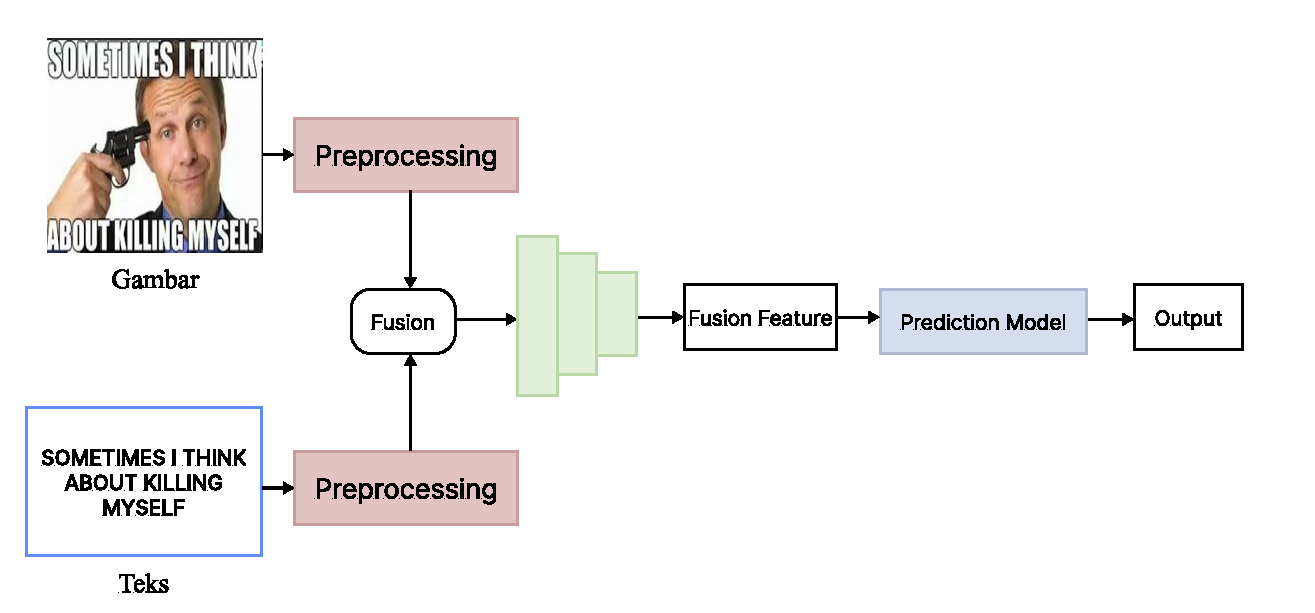
\includegraphics[width=0.9\textwidth]{figure/early.pdf}
\caption{Contoh \textit{Early Fusion}}
\label{fig:4.earlyfusion}
\end{figure}

Pada pendekatan ini, modalitas digabungkan pada tingkat input sebelum proses \textit{encoding}. Contohnya pada Gambar \ref{fig:4.earlyfusion}, data gambar dan teks digabung menjadi satu representasi gabungan yang kemudian diberikan ke \textit{neural network}. \textit{Early fusion} memungkinkan model mempelajari interaksi antar-modalitas dari tahap awal, tetapi menghadapi tantangan signifikan karena heterogenitas struktur data misalnya perbedaan dimensi, skala, dan format yang dapat menyulitkan integrasi langsung \cite{baltrusaitis2019multimodal}. \par

\subsubsection{\textit{Intermediate Fusion}} \label{II.teori8.2}
\begin{figure}[H]
\centering
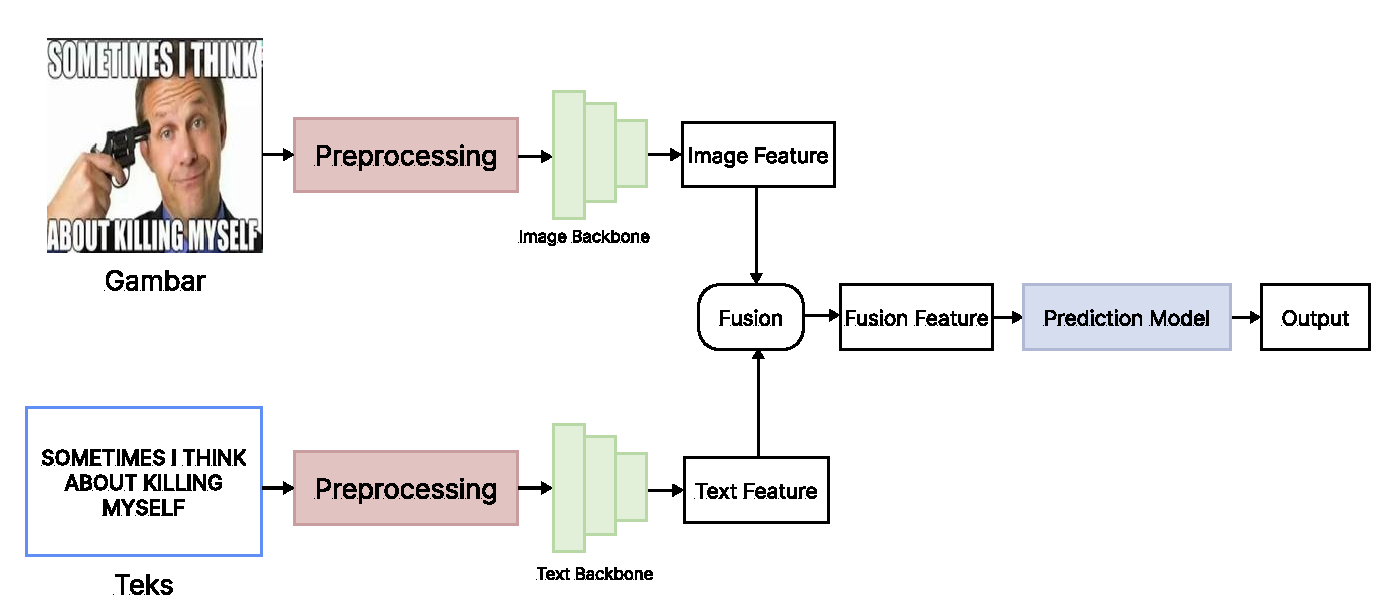
\includegraphics[width=0.9\textwidth]{figure/intermediate.pdf}
\caption{Contoh \textit{Intermediate Fusion}}
\label{fig:5.intermediatefusion}
\end{figure}  
Pada Gambar \ref{fig:5.intermediatefusion}, setiap modalitas terlebih dahulu diproses oleh \textit{encoder} masing-masing untuk menghasilkan \textit{embedding} atau fitur spesifik modalitas. Setelah itu, \textit{embedding} dari berbagai modalitas digabung misalnya melalui \textit{concatenation}, \textit{projection}, \textit{pooling}, atau mekanisme \textit{fusion} lanjutan sebelum diteruskan ke lapisan prediksi. Pendekatan ini menawarkan keseimbangan antara kemampuan merepresentasikan keunikan tiap modalitas dan mempelajari hubungan lintas-modalitas, sehingga banyak digunakan pada model modern, termasuk sistem vision language \cite{jiao2024comprehensive}. \par

\subsubsection{\textit{Late Fusion}} \label{II.teori8.3}
\begin{figure}[H]
\centering
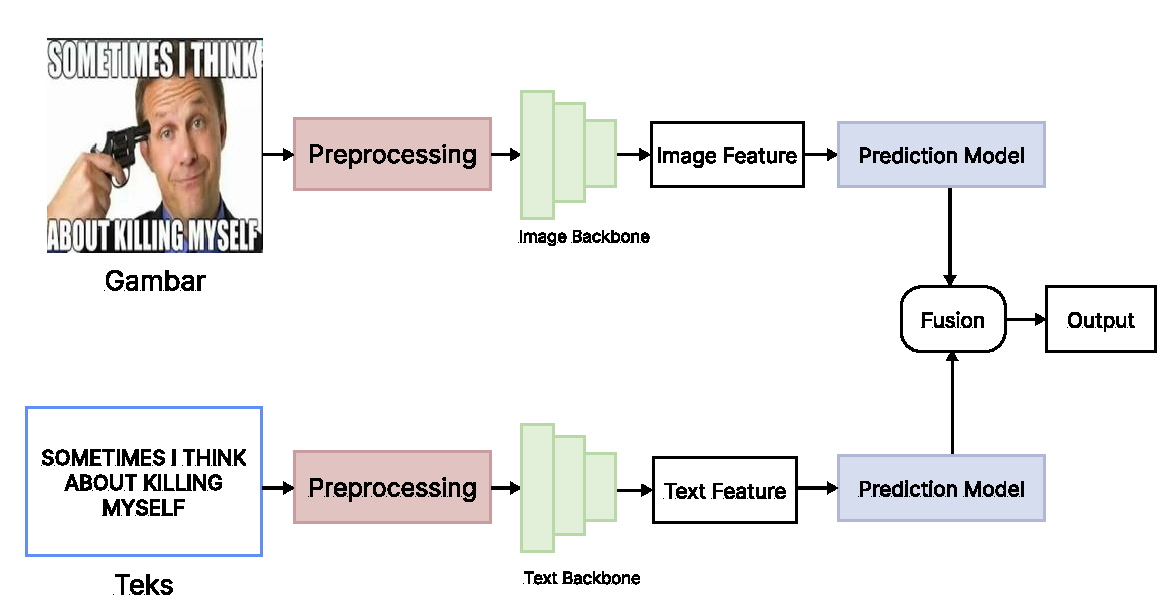
\includegraphics[width=0.9\textwidth]{figure/late.pdf}
\caption{Contoh \textit{Late Fusion}}
\label{fig:6.latefusion}
\end{figure} 
Pada Gambar \ref{fig:6.latefusion} setiap modalitas diproses secara independen hingga menghasilkan prediksi masing-masing, seperti probabilitas atau skor klasifikasi. Prediksi tersebut kemudian digabung menggunakan metode seperti \textit{weighted sum}, \textit{voting}, atau \textit{averaging} untuk memperoleh prediksi akhir. \textit{Late fusion} efektif ketika modalitas relatif independen dan prediksi masing-masing sudah cukup kuat, namun kurang mampu menangkap interaksi semantik yang mendalam antar-modalitas \cite{jiao2024comprehensive}. \par

\subsubsection{\textit{Hybrid Fusion}} \label{II.teori8.4}
\begin{figure}[H]
\centering
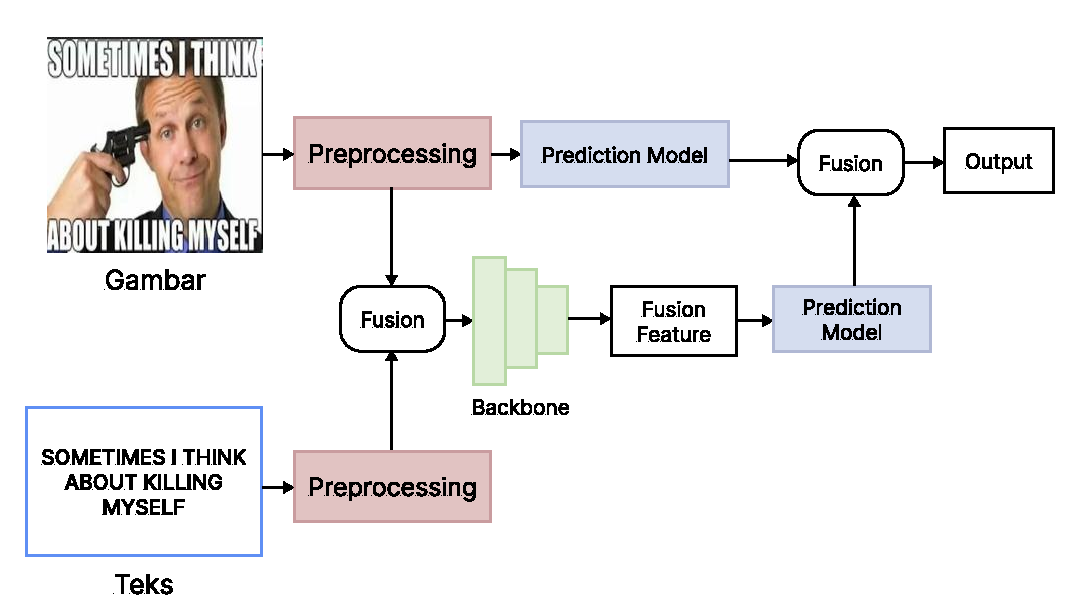
\includegraphics[width=0.9\textwidth]{figure/hybrid.pdf}
\caption{Contoh \textit{Hybrid Fusion}}
\label{fig:7.hybridfusion}
\end{figure}
\textit{Hybrid fusion} menggabungkan dua atau lebih strategi \textit{fusion}, misalnya mengombinasikan \textit{feature-level fusion} dan \textit{decision-level fusion}, atau menggabungkan \textit{embedding} dengan mekanisme \textit{attention} sekaligus memanfaatkan penggabungan skor prediksi. Pada Gambar \ref{fig:7.hybridfusion}, \textit{hybrid fusion} banyak digunakan pada aplikasi multimodal yang kompleks karena mampu memanfaatkan kelebihan beragam strategi sekaligus mengatasi keterbatasan masing-masing \cite{jiao2024comprehensive}. Dalam praktiknya, pemilihan teknik \textit{fusion} sangat bergantung pada karakteristik data, tujuan aplikasi, serta kompleksitas model yang diinginkan. Pendekatan \textit{intermediate fusion} sering kali menjadi pilihan populer karena fleksibilitas dan kemampuannya dalam menangkap hubungan lintas-modalitas secara efektif. 


\subsection{Metode \textit{Fusion} dalam Multimodal \textit{Learning}} \label{II.teori8.5}
Dalam multimodal\textit{learning}, proses \textit{fusion} merupakan tahap penting untuk menggabungkan representasi dari berbagai modalitas, seperti teks dan gambar, menjadi satu representasi terpadu. Berbagai metode \textit{fusion} telah dikembangkan untuk menangkap hubungan antar modalitas dengan tingkat kompleksitas yang berbeda. Pemilihan metode \textit{fusion} yang tepat dapat mempengaruhi kemampuan model dalam memahami interaksi antar fitur serta performa klasifikasi yang dihasilkan \cite{baltrusaitis2018multimodal}.

\subsubsection{\textit{Concatenation Fusion}}
\textit{Concatenation fusion} merupakan metode paling sederhana dalam menggabungkan fitur dari dua modalitas dengan cara menggabungkan vektor fitur secara langsung menjadi satu representasi. Metode ini tidak melakukan transformasi tambahan terhadap fitur, sehingga mempertahankan informasi asli dari masing-masing modalitas. Meskipun sederhana, metode ini sering digunakan karena efektif dan tidak menambah kompleksitas model secara signifikan \cite{ngiam2011multimodal}. Secara matematis, \textit{concatenation fusion} dapat dituliskan sebagai berikut:

\begin{equationcaptioned}[eq:concatenation-fusion]{
	z = [x ; y]
}{
	Perhitungan \textit{Concatenation Fusion}
}
\end{equationcaptioned}

\noindent
\text{Keterangan:}

\begin{tabular}{l l}
$x$      & : fitur teks \\
$y$      & : fitur gambar \\
$z$      & : vektor fitur hasil penggabungan \\
$[\,;\,]$ & : operasi \textit{concatenation} \\
\end{tabular} \\

\subsubsection{\textit{Addition} dan \textit{Multiplication Fusion}} 
\textit{Addition} dan \textit{multiplication fusion} merupakan metode penggabungan fitur secara \textit{element-wise}. Pada \textit{addition fusion}, nilai fitur dari kedua modalitas dijumlahkan, sedangkan pada \textit{multiplication fusion} dilakukan perkalian antar elemen fitur. Metode ini lebih sederhana dibandingkan pendekatan lainnya, namun memiliki keterbatasan dalam menangkap hubungan kompleks antar modalitas karena hanya mengandalkan operasi dasar \cite{kiela2019supervised}.

\begin{equationcaptioned}[eq:addition-fusion]{
	z = x + y
}{
	Rumus \textit{Addition Fusion}
}
\end{equationcaptioned}

\begin{equationcaptioned}[eq:multiplication-fusion]{
	z = x \odot y
}{
	Rumus \textit{Multiplication Fusion}
}
\end{equationcaptioned}

\noindent
\text{Keterangan:}

\begin{tabular}{l l}
$x$ & : vektor fitur dari modalitas pertama \\
$y$ & : vektor fitur dari modalitas kedua \\
$z$ & : representasi fitur hasil \textit{fusion} \\
$+$ & : operasi penjumlahan elemen per elemen \\
$\odot$ & : operasi perkalian elemen per elemen \\
\end{tabular}

\subsubsection{\textit{Gated Fusion}}
\textit{Gated fusion} merupakan metode \textit{fusion} yang menggunakan mekanisme gerbang (\textit{gate}) untuk mengatur seberapa besar kontribusi masing-masing modalitas terhadap representasi akhir. Melalui fungsi aktivasi seperti \textit{sigmoid}, model dapat mempelajari bobot adaptif untuk menentukan apakah informasi dari teks atau gambar lebih dominan dalam tertentu. Pendekatan ini membuat proses \textit{fusion} lebih fleksibel dibandingkan metode sederhana karena mampu menyesuaikan kontribusi tiap modalitas secara dinamis \cite{arevalo2017gated}.
\\

\begin{equationcaptioned}[eq:gated-fusion]{
\begin{aligned}
g &= \sigma(Wx + b) \\
z &= g \odot x + (1 - g) \odot y
\end{aligned}
}{
Rumus \textit{Gated Fusion}
}
\end{equationcaptioned}

\noindent
\text{Keterangan:}

\begin{tabular}{l l}
$x$ & : vektor fitur dari modalitas pertama \\
$y$ & : vektor fitur dari modalitas kedua \\
$W$ & : matriks bobot yang dipelajari model \\
$b$ & : \textit{bias} \\
$g$ & : nilai \textit{gate} atau bobot kontribusi modalitas \\
$\sigma$ & : fungsi aktivasi \textit{sigmoid} \\
$z$ & : representasi fitur hasil \textit{fusion} \\
$\odot$ & : operasi perkalian elemen per elemen \\
\end{tabular} \\

\subsubsection{\textit{Bilinear Fusion}}
\textit{Bilinear fusion} merupakan metode yang digunakan untuk menangkap interaksi non-linear antara dua modalitas dengan memodelkan hubungan pasangan fitur secara lebih kaya. Berbeda dari \textit{fusion} sederhana, metode ini mempertimbangkan hubungan silang antara setiap elemen fitur dari dua modalitas, sehingga mampu menghasilkan representasi yang lebih ekspresif. Namun, pendekatan ini umumnya membutuhkan kompleksitas komputasi yang lebih tinggi \cite{fukui2016multimodal}.

\begin{equationcaptioned}[eq:bilinear-fusion]{
	z = x^{T}Wy
}{
	Rumus \textit{Bilinear Fusion}
}
\end{equationcaptioned}

\noindent
\text{Keterangan:}

\begin{tabular}{l l}
$x$ & : vektor fitur dari modalitas pertama \\
$y$ & : vektor fitur dari modalitas kedua \\
$W$ & : matriks bobot bilinear yang dipelajari model \\
$x^{T}$ & : transpose dari vektor fitur $x$ \\
$z$ & : representasi hasil \textit{fusion bilinear} \\
\end{tabular}


\subsection{\textit{Projection Layer} pada Model Multimodal} \label{II.teori8.6}
\textit{Projection layer} merupakan lapisan tambahan dalam arsitektur \textit{deep learning} yang berfungsi untuk memetakan representasi fitur dari suatu ruang ke ruang lain dengan dimensi tertentu. Lapisan ini umumnya digunakan untuk menyesuaikan dimensi fitur, menyederhanakan representasi, atau menyelaraskan fitur agar dapat digunakan pada tahap pemrosesan selanjutnya \cite{articleheaton2017}. Dalam \textit{deep learning}, fitur yang dihasilkan oleh suatu \textit{encoder} atau jaringan sebelumnya sering kali memiliki dimensi yang tidak sesuai dengan kebutuhan model berikutnya. Oleh karena itu, \textit{projection layer} digunakan untuk mentransformasikan fitur tersebut ke dalam ruang representasi baru yang lebih sesuai, baik dari segi dimensi maupun distribusi \cite{inbookbishop2006}.

Salah satu bentuk normalisasi yang umum digunakan adalah \textit{L2 normalization}, yang dirumuskan sebagai:

\begin{equationcaptioned}[eq:l2-norm-projection]{
\hat{z} = \frac{z}{\|z\|}
}{
Rumus \textit{L2 Normalization}
}
\end{equationcaptioned}

\noindent
\text{Keterangan:}

\begin{tabular}{l l}
$\hat{z}$ & : vektor hasil normalisasi \\
$\|z\|$ & : norma L2 dari vektor $z$ \\ 
\end{tabular}
\vspace{0.5cm}

\indent Normalisasi ini menghasilkan vektor dengan panjang satu (\textit{unit vector}), sehingga lebih stabil digunakan dalam berbagai operasi seperti perhitungan jarak atau kesamaan antar fitur. Selain itu, dalam beberapa aplikasi, terutama yang melibatkan perbandingan antar representasi, digunakan ukuran kesamaan seperti \textit{cosine similarity} yang dirumuskan sebagai:

\begin{equationcaptioned}[eq:cosine-sim-projection]{
\text{sim}(z_1, z_2) = \frac{z_1 \cdot z_2}{\|z_1\|\,\|z_2\|}
}{
Rumus \textit{Cosine Similarity}
}
\end{equationcaptioned}

\noindent
\text{Keterangan:}

\begin{tabular}{l l}
$z_1, z_2$ & : dua vektor yang dibandingkan \\
$\cdot$ & : operasi \textit{dot product} \\
$\|z_1\|, \|z_2\|$ & : norma L2 masing-masing vektor \\
\end{tabular}
\vspace{0.5cm}

\indent Dengan demikian, \textit{projection layer} berperan penting dalam proses pembelajaran representasi (\textit{representation learning}), karena memungkinkan model untuk mengubah dan menyesuaikan fitur agar lebih relevan terhadap tugas yang dihadapi.

\subsection{\textit{Computer Vision}} \label{II.teori2}
\textit{Computer vision} merupakan bidang dalam kecerdasan buatan yang berfokus pada bagaimana mesin dapat memahami dan menafsirkan informasi visual dari gambar maupun video melalui representasi numerik yang terstruktur \cite{sciencedirect_computer_vision_overview}. Proses komputasional ini mencakup tahapan seperti ekstraksi fitur, deteksi pola, dan pemahaman objek melalui algoritma yang mempelajari hubungan spasial maupun semantik di dalam citra. Pendekatan modern dalam \textit{computer vision} didominasi oleh \textit{deep learning}, khususnya \textit{Convolutional Neural Networks} (CNN), yang mampu mempelajari fitur visual secara hierarkis mulai dari tepi (\textit{low-level features}) hingga representasi abstrak (\textit{high-level features}) melalui pembelajaran berbasis data \cite{lecun2015deep}. Perkembangan lebih lanjut \textit{Vision Transformer} (ViT), arsitektur berbasis mekanisme \textit{self-attention} yang memecah gambar dalam bentuk \textit{patch} dan memprosesnya seperti token dalam \textit{natural language processing}, sehingga menghasilkan performa kompetitif pada skala data besar \cite{dosovitskiy2020image}. Dengan kemampuan menghasilkan \textit{embedding} visual yang kaya semantik, \textit{computer vision}  menjadi fondasi penting dalam berbagai aplikasi, termasuk klasifikasi gambar, deteksi objek, dan pemahaman multimodal seperti pada model \textit{vision-language}.

\subsection{\textit{Natural Language Processing} } \label{II.teori3}
\textit{Naural language processing} merupakan cabang kecerdasan buatan yang berfokus pada bagaimana mesin dapat memahami, memproses, dan menghasilkan bahasa manusia melalui representasi matematis yang terstruktur \cite{jurafsky2026slp}. NLP modern bertumpu pada pembelajaran representasi \textit{(representation learning)}, dimana teks diubah menjadi \textit{embedding} yang mampu menangkap konteks semantik maupun sintaksis \cite{liu2018neural}. Pergeseran besar dalam NLP terjadi dengan hadirnya pendekatan berbasis \textit{deep learning}, yang dimulai dengan penggunaan \textit{recurrent neural networks} (RNN) dan \textit{Long Short-Term Memory} (LSTM), sebelum akhirnya banyak digantikan oleh arsitektur Transformer yang memungkinkan pemodelan konteks panjang melalui mekanisme \textit{self-attention} \cite{young2017recent}. Transformer kemudian menjadi fondasi model-model pra-latih (\textit{pre-trained models}) seperti BERT, GPT, dan ELECTRA yang memanfaatkan \textit{pre-training} berskala besar untuk mempelajari pola bahasa secara mendalam, sehingga meningkatkan performa berbagai tugas seperti klasifikasi teks, analisis sentimen, dan pemahaman multimodal \cite{devlin2018bert}. Dengan kemampuan menghasilkan representasi linguistik yang kaya konteks, NLP menjadi komponen penting dalam pemrosesan modalitas teks pada sistem multimodal modern. \par


\subsection{\textit{Deep Learning}} \label{II.teori1}
\textit{Deep learning} merupakan pendekatan dalam \textit{machine learning} yang menggunakan jaringan saraf tiruan berlapis banyak \textit{(deep neural networks)} untuk mempelajari pola dan representasi data secara otomatis melalui proses hierarkis. Berbeda dari metode pembelajaran tradisional yang mengandalkan rekayasa fitur manual, \textit{deep learning} memungkinkan ekstraksi fitur kompleks secara langsung dari data mentah menggunakan transformasi non-linear yang dioptimalkan melalui algoritma \textit{backpropagation} \cite{lecun2015deep}. Konsep representasi berlapis inilah yang membuat \textit{deep learning} unggul dalam menangani data dengan skala besar dengan struktur yang beragam seperti teks dan gambar karena model dapat mempelajari fitur tingkat rendah hingga abstraksi tingkat tinggi secara bertahap \cite{schmidhuber2015deep}. Dengan fleksibilitas dan kemampuan generalisasi yang kuat, \textit{deep learning} telah menjadi fondasi utama pengembangan berbagai arsitektur modern dalam bidang \textit{computer vision} dan pemrosesan bahasa alami. Salah satu arsitektur \textit{deep learning} yang banyak digunakan dalam pemrosesan data sekuensial seperti teks adalah Transformer \cite{Hakim2025DeteksiBeritaPalsu}.


\subsection{Transformer} \label{II.teori4}
Transformer merupakan salah satu arsitektur \textit{deep learning} yang diperkenalkan oleh Vaswani \textit{et al}. pada tahun 2017 dan menjadi dasar bagi berbagai model bahasa dan multimodal modern. Transformer terdiri dari beberapa layer encoder yang disusun secara berulang. Setiap layer terdiri dari dua komponen utama, yaitu \textit{multi-head self-attention} untuk menangkap hubungan antar token, serta \textit{feed-forward network} untuk memproses representasi fitur. Selain itu, digunakan \textit{residual connection} dan \textit{layer normalization} untuk menjaga stabilitas pelatihan model.

Salah satu komponen penting dalam Transformer adalah \textit{multi-head attention}, yang memungkinkan model untuk memproses informasi dari berbagai subruang representasi secara paralel. Setiap token direpresentasikan sebagai vektor, kemudian dihitung nilai \textit{attention} berdasarkan interaksi antara \textit{query (Q)}, \textit{key (K)}, dan \textit{value (V)}. Proses ini menggunakan rumus \textit{Scaled Dot-Product Attention} yang dihitung sebagai berikut:

\begin{equationcaptioned}[eq:scaled-attention]{
	\mathrm{Attention}(Q, K, V) = \mathrm{softmax}\left( \frac{QK^{T}}{\sqrt{d_k}} \right) V
}{
	\textit{Scaled Dot-Product Attention}
}
\end{equationcaptioned}

\noindent
\text{Keterangan:}

\begin{tabular}{l l}
$Q$      & : \textit{query} \\
$K$      & : \textit{key} \\
$V$      & : \textit{value} \\
$d_k$    & : dimensi \textit{key} \\
$QK^T$   & : \textit{dot-product} \textit{query} dan \textit{key} \\
\textit{softmax} & : fungsi normalisasi \\
\end{tabular} \\

Selain itu, \textit{multi-head attention} memungkinkan model untuk memproses informasi dari berbagai subruang representasi, yang mendukung pengolahan informasi dalam skala besar dan memungkinkan penanganan konteks yang lebih kompleks.

\begin{figure}[H]
	\centering
	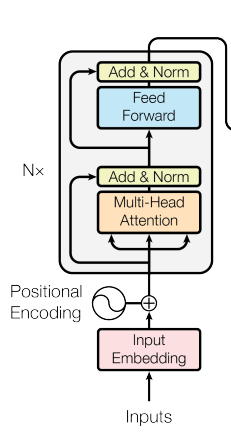
\includegraphics[width=0.35\textwidth]{figure/Arsitektur Transformer.png}
	\caption{Arsitektur Transformer dengan \textit{Encoder} \cite{vaswani2017attention}}
	\label{fig:2.transformer}
	% {\footnotesize Sumber: Vaswani et al., 2017}
\end{figure}

Gambar \ref{fig:2.transformer} menunjukkan arsitektur Transformer dengan \textit{encoder} yang fokus pada bagian \textit{input embedding}. Proses dimulai dengan input yang berupa urutan token, yang kemudian diproses menjadi \textit{input embedding}. \textit{Input embedding} mengubah token-token dalam urutan menjadi vektor representasi yang dapat diproses oleh model. Vektor-vektor ini kemudian diperkaya dengan \textit{positional encoding} untuk mempertahankan informasi urutan input, yang sangat penting dalam model Transformer yang tidak bergantung pada urutan sekuensial.
Gambar ini menggambarkan bagaimana \textit{input embedding} berfungsi sebagai representasi awal bagi setiap token yang masuk, dan bagaimana \textit{embedding} ini bekerja bersama dengan komponen lain seperti \textit{multi-head attention} untuk menghasilkan representasi yang lebih kompleks dalam proses pemodelan \cite{vaswani2017attention}. Kemampuan Transformer dalam menangkap hubungan konteks yang kompleks ini menjadikannya fondasi utama dalam pengembangan model multimodal dan model bahasa modern. Perkembangan arsitektur Transformer ini kemudian mendorong lahirnya berbagai model multimodal yang mampu mengintegrasikan informasi visual dan tekstual, salah satunya adalah CLIP.

\subsection{\textit{Contrastive Language-Image Pre-training} } \label{II.teori5}
\textit{Contrastive Language--Image Pre-training} (CLIP) adalah model \textit{vision--language} yang dikembangkan oleh OpenAI untuk mempelajari keterkaitan semantik antara gambar dan teks melalui pembelajaran kontrasif berskala besar. CLIP terdiri atas dua \textit{encoder} terpisah, yaitu \textit{image encoder} berbasis ViT, serta \textit{text encoder} berbasis Transformer yang keduanya memetakan gambar dan teks ke dalam ruang \textit{embedding} yang sama. Selama pelatihan, CLIP memanfaatkan 400 juta pasangan gambar--teks dari internet untuk mempelajari \textit{alignment} antar-modalitas dengan menempatkan pasangan yang cocok semakin dekat dan pasangan tidak cocok semakin jauh dalam ruang vektor. Mekanisme pembelajaran ini diformalkan menggunakan InfoNCE (\textit{contrastive loss}), yang dirumuskan sebagai:
\begin{equationcaptioned}[eq:clip-infoNCE]{
\begin{aligned}
\mathcal{L} = -\frac{1}{2N} \sum_{i=1}^{N} \Bigg[
	&\log \frac{\exp(\cos(f_I(L_i), f_T(T_i))/\tau)}{\sum_{j=1}^{N} \exp(\cos(f_I(L_i), f_T(T_j))/\tau)} \\
	+ &\log \frac{\exp(\cos(f_T(T_i), f_I(L_i))/\tau)}{\sum_{j=1}^{N} \exp(\cos(f_T(T_i), f_I(L_j))/\tau)}
\Bigg]
\end{aligned}
}{InfoNCE (\textit{Contrastive Loss}) pada CLIP}
\end{equationcaptioned}

\noindent
\text{Keterangan:}

\begin{tabular}{l l}
$\mathcal{L}$ & : fungsi \textit{contrastive loss} \\ 
$N$ & : jumlah pasangan data dalam satu \textit{batch} \\  
$L_i$ & : citra ke-$i$ \\ 
$T_i$ & : teks ke-$i$ yang berpasangan dengan $L_i$ \\ 
$f_I(\cdot)$ & : fungsi \textit{encoder} citra \\ 
$f_T(\cdot)$ & : fungsi \textit{encoder} teks \\ 
$\cos(\cdot,\cdot)$ & : \textit{cosine similarity} \\ 
$\tau$ & : parameter temperatur \\ 
$\exp(\cdot)$ & : fungsi eksponensial \\ 
$\sum_{j=1}^{N}$ & : jumlah seluruh sampel dari 1 hingga N dalam satu \textit{batch} \\ 
\end{tabular} \\

Gambar \ref{fig:3.clip} di bawah ini mengilustrasikan arsitektur model CLIP yang menerapkan mekanisme dual-encoder untuk mempelajari representasi visual dan tekstual secara bersamaan. Dalam proses ini, \textit{text encoder} dan \textit{image encoder} bekerja secara paralel mengubah sekumpulan input gambar dan teks menjadi vektor fitur \textit{(embedding)} dalam ruang dimensi yang sama. Setiap pasangan gambar-teks yang sesuai dipetakan ke vektor yang berdekatan, sementara pasangan yang tidak sesuai dipisahkan lebih jauh, melalui optimasi fungsi InfoNCE yang memaksimalkan kesamaan kosinus antar \textit{embedding} \cite{Pan2022ContrastiveKCLIP}. 

\begin{figure}[H]
	\centering
	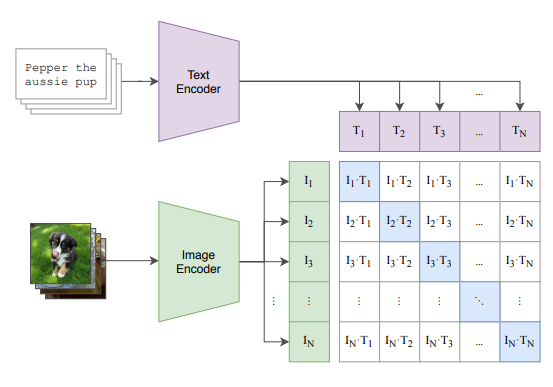
\includegraphics[width=0.7\textwidth]{figure/CLIP.png}
	\caption{Arsitektur CLIP \cite{Pan2022ContrastiveKCLIP}}
	\label{fig:3.clip}
	% {\footnotesize Sumber: Vaswani et al., 2017}
\end{figure}

CLIP digunakan sebagai ekstraksi fitur gambar \textit{image encoder}, karena kemampuannya dalam memahami representasi visual yang selaras dengan konteks semantik. Selain digunakan dalam model multimodal seperti CLIP, arsitektur Transformer juga menjadi dasar bagi berbagai model bahasa modern yang digunakan untuk memproses teks secara lebih mendalam. Salah satu model tersebut adalah ELECTRA.

\subsection{\textit{Efficiently Learning an Encoder that Classifies Token Replacements Accurately} } \label{II.teori6}

\textit{Efficiently Learning an Encoder that Classifies Token Replacements Accurately} (ELECTRA)merupakan model pra-latih berbasis arsitektur Transformer yang diperkenalkan sebagai alternatif yang lebih efisien dibandingkan pendekatan \textit{Masked Language Modeling} (MLM) seperti pada BERT. Berbeda dengan MLM yang hanya mempelajari representasi dari token yang di-\textit{masking}, ELECTRA menggunakan pendekatan diskriminatif yang disebut \textit{Replaced Token Detection} (RTD), di mana model dilatih untuk membedakan apakah suatu token dalam urutan merupakan token asli atau hasil penggantian oleh model \textit{generator} \cite{clark2020electra}.

Arsitektur ELECTRA terdiri dari dua komponen utama, yaitu \textit{generator} dan \textit{discriminator}. \textit{Generator} bertugas menghasilkan token pengganti berdasarkan skema MLM dalam skala kecil, sedangkan \textit{discriminator} berfungsi untuk mengevaluasi setiap token dalam urutan dan menentukan apakah token tersebut merupakan token asli atau hasil substitusi. Dengan pendekatan ini, proses pembelajaran terjadi pada seluruh token dalam satu urutan, tidak terbatas hanya pada token tertentu seperti pada \textit{mask language modelling}. Gambar \ref{fig:3.electra} di bawah ini menunjukkan arsitektur ELECTRA yang terdiri dari interaksi antara \textit{generator} dan \textit{discriminator} dalam proses pelatihan. Melalui mekanisme ini, ELECTRA mampu mempelajari konteks bahasa secara lebih menyeluruh dibandingkan pendekatan pra-latih tradisional.

\begin{figure}[H]
	\centering
	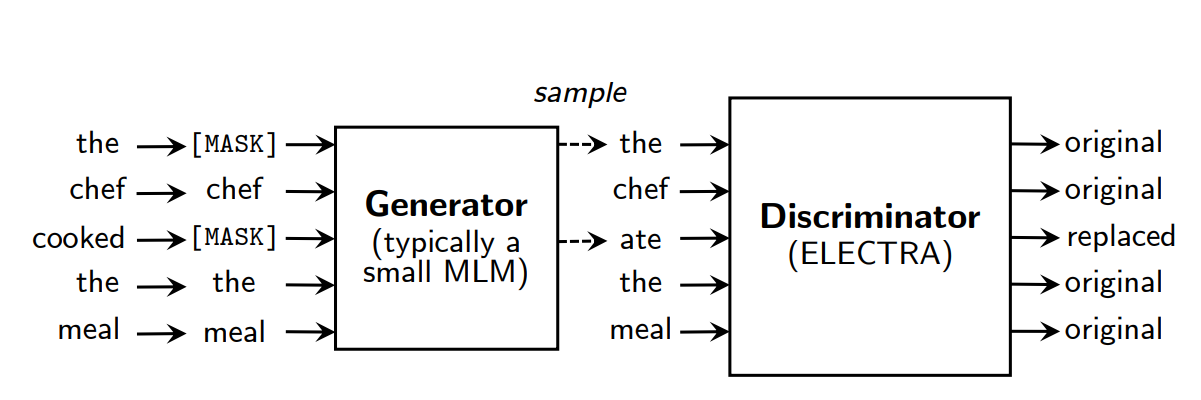
\includegraphics[width=0.7\textwidth]{figure/ELECTRA.png}
	\caption{Arsitektur ELECTRA \cite{clark2020electra}}
	\label{fig:3.electra}
\end{figure}

Proses pelatihan ELECTRA dimodelkan melalui fungsi RTD  \textit{loss} sebagai berikut: 
\\

\begin{equationcaptioned}[eq:rtd-loss]{
\mathcal{L}_{\text{RTD}} = - \sum_{i=1}^{n} \left[ y_i \log D(x_i) + (1 - y_i)\log \left(1 - D(x_i)\right) \right]
}{\textit{Replaced Token Detection} \textit{Loss} pada ELECTRA}
\end{equationcaptioned}

\noindent
\text{Keterangan:}

\begin{tabular}{l l}
$\mathcal{L}_{RTD}$ & : fungsi \textit{Replaced Token Detection loss} \\ 
$n$ & : jumlah token dalam satu \textit{batch} \\ 
$i$ & : indeks \textit{token} \\
$x_i$ & : \textit{token} ke-$i$ \\
$y_i$ & : label \textit{token} (0: asli, 1: hasil penggantian) \\
$D(x_i)$ & : probabilitas bahwa \textit{token} $x_i$ adalah hasil penggantian \\
$\log$ & : fungsi logaritma \\ 
\end{tabular} \\

dengan $y_i = 1$ jika \textit{token} merupakan \textit{token} asli dan $y_i = 0$ jika \textit{token} merupakan hasil penggantian, serta $D(x_i)$ merupakan probabilitas bahwa \textit{token} tersebut adalah \textit{token} asli. Fungsi \textit{loss} ini mendorong model untuk mempelajari representasi kontekstual yang mampu membedakan distribusi \textit{token} asli dan \textit{token} hasil substitusi secara efektif. Pendekatan RTD memungkinkan ELECTRA menjadi lebih \textit{sample-efficient} dibandingkan model berbasis MLM, karena seluruh \textit{token} dalam urutan digunakan dalam proses pembelajaran. Hal ini menjadikan ELECTRA lebih efisien secara komputasi sekaligus mampu menghasilkan representasi linguistik yang lebih kaya dan informatif. Dibandingkan dengan BERT, ELECTRA memiliki keunggulan dalam efisiensi pelatihan dan pemanfaatan data, sehingga lebih efektif digunakan pada dataset dengan ukuran terbatas. Selain itu, kemampuan model dalam mengevaluasi setiap \textit{token} berdasarkan konteks global menjadikannya cocok untuk tugas klasifikasi teks yang membutuhkan pemahaman kontekstual yang mendalam.

Dalam penelitian ini, ELECTRA digunakan sebagai \textit{text encoder} karena kemampuannya dalam menghasilkan representasi teks yang efisien dan kontekstual. 
Selain itu, pemilihan ELECTRA juga didasarkan pada ketersediaan model pra-latih yang telah dilatih pada domain teks yang mengandung sinyal \textit{suicidality} atau \textit{self-harm} \cite{sentinet_suicidality}. Model pra-latih pada domain spesifik ini memungkinkan representasi tekstual yang lebih relevan terhadap konteks penelitian, karena telah memiliki pemahaman awal terhadap pola bahasa yang berkaitan dengan ekspresi emosional dan indikasi \textit{self-harm}. Dengan demikian, penggunaan model ini diharapkan dapat meningkatkan kemampuan sistem dalam mendeteksi meme \textit{self-harm} secara lebih akurat.


\subsection{\textit{Pre-processing} Data} \label{II.teori11}
\textit{Pre-processing} data adalah tahap penting  yang bertujuan untuk menyiapkan data mentah agar siap digunakan dalam model. Tahap prapemrosesan data terdiri dari berbagai teknik yang masing-masing dirancang untuk mempersiapkan data dalam bentuk yang sesuai untuk analisis lebih lanjut. Berikut adalah beberapa teknik prapemrosesan data yang digunakan dalam penelitian ini.


\subsubsection{\textit{Resize} Gambar} \label{II.teori11.1}
\textit{Resize} gambar adalah proses mengubah ukuran gambar untuk memenuhi kebutuhan model yang digunakan. Secara matematis, proses ini melibatkan perhitungan rasio antara dimensi gambar awal dan ukuran target. Jika ukuran gambar asli adalah $(W, H)$ dan gambar yang diinginkan berukuran $(W', H')$, maka rasio skala untuk lebar dan tinggi adalah sebagai berikut: 
\\

\begin{equationcaptioned}[eq:scale-factor]{
	\text{\textit{Scale Factor}} = \left( \frac{W'}{W} \right) \left( \frac{H'}{H} \right)
}{
Perhitungan Faktor Skala
}
\end{equationcaptioned}

\noindent
\text{Keterangan:}

\begin{tabular}{l l}
$\text{\textit{Scale Factor}}$ & : faktor skala perubahan ukuran gambar \\ 
$W$ & : lebar asli gambar (\textit{width}) \\ 
$H$ & : tinggi asli gambar (\textit{height}) \\ 
$W'$ & : lebar gambar setelah diubah ukurannya \\ 
$H'$ & : tinggi gambar setelah diubah ukurannya \\ 

\end{tabular} \\

\textit{Resize} gambar akan mengubah ukuran citra asli berdasarkan skala ini, yang dapat memperkecil atau memperbesar citra sesuai dengan ukuran yang diinginkan. Dengan memperkecil ukuran gambar, kita dapat mengurangi jumlah parameter yang perlu diproses, meningkatkan efisiensi, dan mengurangi waktu komputasi \cite{Xu2023ImageAugmentationSurvey}.

% \subsubsection{Normalisasi Gambar} \label{II.teori11.2}
% CLIP (\textit{Contrastive Language--Image Pretraining}) menerapkan normalisasi pada dua tahapan krusial dalam arsitekturnya. Pertama, normalisasi input gambar dilakukan dengan menstandarisasi nilai piksel menggunakan \textit{mean} ($\mu$) dan standar deviasi ($\sigma$) spesifik agar distribusi data selaras dengan \textit{backbone encoder} visual (seperti ResNet atau ViT). Secara matematis, transformasi ini dapat dituliskan sebagai:

% \begin{equationcaptioned}[eq:input_norm]{
% 	x_{norm} = \frac{x - \mu}{\sigma}
% }{
% Normalisasi Input Gambar
% }
% \end{equationcaptioned}

% dimana $x$ adalah nilai piksel asli dan $x_{norm}$ adalah input yang diteruskan ke jaringan. 

% Kedua, setelah citra dan teks diproses menjadi \textit{embedding}, CLIP menerapkan \textit{L2-normalization} pada vektor tersebut agar diproyeksikan ke dalam \textit{unit hypersphere}. Jika $v$ adalah vektor fitur keluaran dari \textit{encoder}, maka normalisasi didefinisikan sebagai:

% \begin{equationcaptioned}[eq:l2_norm]{
% 	v_{norm} = \frac{v}{\|v\|_2} = \frac{v}{\sqrt{\sum_{i=1}^{d} v_i^2}} + h
% }{
% Normalisasi Vektor
% }
% \end{equationcaptioned}

% Normalisasi vektor pada persamaan \ref{eq:l2_norm} ini krusial karena menjadikan operasi \textit{dot product} setara dengan \textit{cosine similarity} dalam perhitungan \textit{loss} kontrastif, sehingga model dapat mempelajari penyelarasan semantik antara teks dan gambar dengan lebih stabil dan konsisten \cite{Pan2022ContrastiveKCLIP}.

\subsubsection{Augmentasi Data} \label{II.teori11.3}
Augmentasi data adalah teknik yang digunakan untuk meningkatkan jumlah dan variasi data pelatihan dengan membuat modifikasi pada data asli \cite{shorten2019survey}. Teknik ini sangat penting dalam pembelajaran mesin, terutama ketika dataset yang tersedia terbatas, karena dapat membantu model untuk belajar lebih baik dan mengurangi risiko \textit{overfitting}. Berikut adalah beberapa teknik augmentasi yang digunakan dalam penelitian ini.

\subsubsubsection{\textit{Flip}} \label{II.teori11.3.1}

\textit{Flip} merupakan salah satu teknik augmentasi data pada citra yang bertujuan untuk meningkatkan keragaman \textit{dataset} dengan cara membalik gambar, baik secara horizontal maupun vertikal. Teknik ini memungkinkan model untuk melihat variasi representasi objek yang sama dari sudut pandang yang berbeda tanpa perlu menambah data baru secara manual. Dengan demikian, model dapat belajar pola yang lebih umum dan tidak terlalu bergantung pada orientasi tertentu dari objek dalam gambar. Penerapan \textit{flip} terbukti membantu meningkatkan kemampuan generalisasi model serta membuatnya lebih \textit{robust} terhadap variasi posisi dan arah objek dalam data \cite{Xu2023ImageAugmentationSurvey}.

\subsubsubsection{\textit{Rotation}} \label{II.teori11.3.2}

\textit{Rotation} merupakan teknik augmentasi yang dilakukan dengan memutar gambar ke kanan atau kiri pada suatu sumbu dengan sudut tertentu, biasanya berada pada rentang 1° hingga 359°. Tingkat keamanan \textit{(safety)} dari augmentasi ini sangat ditentukan oleh besar sudut rotasi, karena rotasi yang terlalu ekstrem dapat menyebabkan hilangnya informasi penting pada citra, seperti tepi objek atau struktur yang relevan \cite{Shorten2019ImageDataAugmentation}.

\subsubsubsection{\textit{Color Jitter}} \label{II.teori11.3.3}

\textit{Color Jitter} merupakan teknik augmentasi data fotometrik yang berfungsi memodifikasi atribut visual citra meliputi kecerahan, kontras, saturasi, dan rona secara stokastik tanpa mengubah struktur geometris objek di dalamnya. Penerapan teknik ini bertujuan untuk mensimulasikan variabilitas pencahayaan yang alami terjadi di dunia nyata, sehingga memaksa model untuk mempelajari fitur struktural yang invarian alih-alih bergantung pada bias warna atau intensitas piksel absolut. Mekanisme distorsi warna ini terbukti efektif dalam meningkatkan kemampuan generalisasi model serta memitigasi risiko \textit{overfitting} akibat keterbatasan variasi visual pada data latih \cite{Shorten2019ImageDataAugmentation}.

\subsection{Evaluasi} \label{II.teori12}
Evaluasi merupakan tahap penting dalam menilai performa model klasifikasi, terutama pada tugas sensitif seperti deteksi konten \textit{self-harm} dalam meme. Evaluasi umumnya dilakukan menggunakan \textit{confusion matrix} yang menggambarkan hubungan antara prediksi model dan kondisi sebenarnya \cite{fawcett2006introduction}. Struktur \textit{confusion matrix} dapat dilihat pada Tabel~\ref{table:confmatrix}.

\begin{table}[H]
	\centering
	\caption{\textit{Confusion Matrix}}
	\label{table:confmatrix}
	\small
	\setlength{\tabcolsep}{4pt}
	\renewcommand{\arraystretch}{1.2}
	\begin{tabular}{>{\centering\arraybackslash}m{2.6cm} >{\centering\arraybackslash}m{1.5cm} >{\centering\arraybackslash}m{1.5cm}}
		\hline
		\textbf{\textit{Actual $\backslash$ Predicted}} & \textbf{\textit{Positive}} & \textbf{\textit{Negative}} \\
		\hline
		\textit{Positive} & TP & FN \\
		\textit{Negative} & FP & TN \\
		\hline
	\end{tabular}
\end{table}

\noindent
\text{Keterangan:}

\begin{tabular}{l l}
TP & : \textit{True Positive}, prediksi positif sesuai dengan kondisi aktual \\ 
TN & : \textit{True Negative}, prediksi negatif sesuai dengan kondisi aktual \\ 
FP & : \textit{False Positive}, prediksi positif namun kondisi aktual negatif \\ 
FN & : \textit{False Negative}, prediksi negatif namun kondisi aktual positif \\ 
\end{tabular} \\

Berdasarkan elemen di atas, beberapa metrik evaluasi dapat dihitung. 
\textit{Accuracy} mengukur proporsi prediksi benar terhadap seluruh sampel, 
namun sering tidak cukup representatif ketika data tidak seimbang 
(\textit{imbalanced}) seperti pada deteksi \textit{self-harm} meme \cite{sokolova2009systematic}. \textit{Precision} mengukur tingkat ketepatan prediksi kelas positif, sedangkan 
\textit{recall} mengukur kemampuan model dalam menangkap seluruh sampel positif. 
Keduanya penting karena kesalahan \textit{false negative} pada deteksi 
konten \textit{self-harm} berpotensi membahayakan pengguna. 
Untuk menyeimbangkan \textit{precision} dan \textit{recall} digunakan \textit{F1-score}, yaitu 
rata-rata harmonik keduanya, yang efektif untuk dataset tidak seimbang 
\cite{powers2020evaluationprecisionrecallfmeasure}. Secara matematis, metrik-metrik evaluasi dirumuskan sebagai berikut:

\begin{equationcaptioned}[eq:accuracy]{
\textit{Accuracy} = 
\frac{TP + TN}{TP + TN + FP + FN}
}{
Perhitungan \textit{Accuracy}
}
\end{equationcaptioned}

\begin{equationcaptioned}[eq:precision]{
\textit{Precision} = 
\frac{TP}{TP + FP}
}{
Perhitungan \textit{Precision}
}
\end{equationcaptioned}

\begin{equationcaptioned}[eq:recall]{
\textit{Recall} = 
\frac{TP}{TP + FN}
}{
Perhitungan \textit{Recall}
}
\end{equationcaptioned}

\begin{equationcaptioned}[eq:f1-score]{
\textit{F1} = 
2 \times 
\frac{
	\textit{Precision} \times \textit{Recall}
}{
	\textit{Precision} + \textit{Recall}
}
}{
Perhitungan \textit{F1-Score}
}
\end{equationcaptioned}

Kombinasi dari seluruh metrik tersebut memberikan gambaran evaluasi yang lebih komprehensif dibandingkan hanya menggunakan \textit{accuracy} saja, terutama karena model untuk deteksi \textit{self-harm} harus sensitif terhadap kesalahan pada kelas positif. 
